% Chapters content

\chapter{Introduction}

\section{Context}

For several years, Carl Haber and his team at Lawrence Berkeley National Laboratory (\gls{lbnl}) have been working on the sound recovery of old mechanical records. They developed two different systems able to extract the sound without any physical contact, using optical methods. These are capable to process many different types of mediums, from early Edison records to vinyl discs, including shellac or lacquer composed discs and others.

Nowadays, a lot of unique and historical records remain in archives from different libraries and museums. They contain some important historical and cultural recordings but as they are aging and deteriorated, it is too delicate to play them with a normal mechanical phonograph. Non-contact feature of optical methods is then important.

The first developed system is called \gls{irene}. It enables to extract the sound using digitized images of the disc. The corresponding program that processes the extraction from the acquisition step is called \gls{rene}.

The second one, \gls{3dprobe}, uses a special probe able to measure the real depth at each position of the scanned record. This gives the best results for certain types of records as the cylinders.

Meanwhile in Switzerland, at the College of Engineering and Architecture of Fribourg, a project called VisualAudio has been developed. It also enables to extract the sound using non-contact optical scanning in a similar manner as \gls{irene}, but it applies not to experimental records such as cylinders.

\section{Project goals}

%Old records can suffer from degradations. One of the most common is known as ``cracked discs''. This problem appears when the lacquer coating shrinks as the disk is getting older. This causes cracks where the underneath hard support is visible, as seen in \autoref{fig:crackeddisc}.
%
%\begin{figure}[!h]
%\centering
%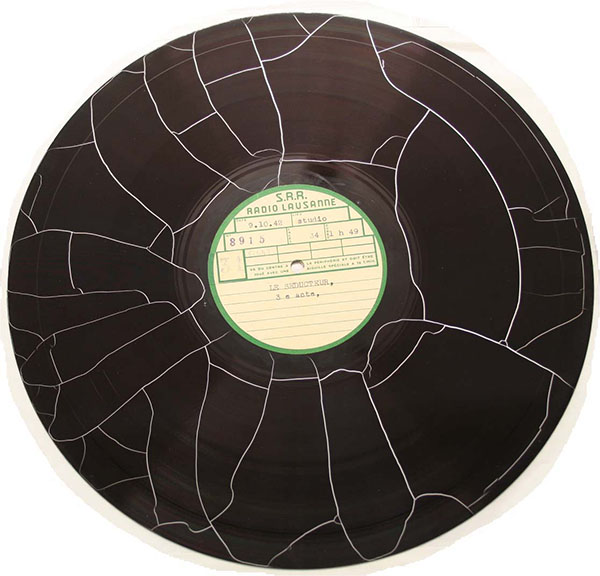
\includegraphics[width=0.7\textwidth]{images/cracked-disc}
%\caption{An example of cracked disc.}
%\label{fig:crackeddisc}
%\end{figure}

Up to now, \gls{irene} and \gls{3dprobe} cannot automatically process these damaged records, because the groove traces are sometimes widely separated and may be shifted from each other. Though a special feature is implemented, enabling the user to manually track the traces, it is not a perfect tool for practical use. Moreover, even with such a feature, it could be really difficult to visually find the correct shifting when the traces look similar.

The aim of this Master's thesis is to find ways to read correctly these kinds of degraded records with the solutions developed at LBNL by Carl Haber and his team. In a first step, an improvement of the manual tracking will be implemented. It is still useful to keep it for some cases, e.g for special early recordings or when a disc is heavily cracked.

Then, the next step will be to design and implement a tracking feature able to process cracked records and link their traces automatically. VisualAudio implements already such a feature. It can then be taken as an example, though it is obviously not possible to directly use its implementation, due to the differences between the systems.

%\section{Report structure}

%TODO This report is separated in...

%\chapter{Acquisition and processing systems}
%
%\section{IRENE}
%
%TODO.
%
%\section{PRISM}
%
%TODO.

%\chapter{Sample recordings}
%
%TODO.

%\chapter{User interface improvements}
%
%TODO.

%\chapter{Tests}
%
%TODO.

%\chapter{Conclusion}
%
%TODO.

%------------------------ Float samples ------------------------

%\begin{figure}[!h]
%\centering
%
\includegraphics[width=0.7\textwidth]{images/logo_lbnl}
%\caption{Image caption.}
%\label{fig:figname}
%\end{figure}

%\begin{table}[!h]
%\begin{center}
%\begin{tabular}{| l c r |}
%    \hline
%    1 & 2 & 3 \\
%    4 & 5 & 6 \\
%    7 & 8 & 9 \\
%    \hline
%\end{center}
%\end{table}

%\begin{lstlisting}[language=C++, caption={Test listing}, label={lst:listingname}]
%// Comment
%int i;
%char c;
%\end{lstlisting}

%\autoref{eq:solve} with variable $s$ such as:
%\begin{equation} \label{eq:solve}
%s = [a_0, (a_0 + a_1), ..., (a_0 + a_1 + ... + a_{n-1})].
%\end{equation}
